\chapter{Feature Sources}\label{sec:features}

A major goal of this work was to introduce rich features into models of human 
pose.  The standard approach is to represent limbs with an edge-based rigid 
template invariant to color, lighting, and minor deformations. In addition to 
this, we use color, shape and geometry. 

In this chapter, we go over feature {\em sources} - the basic channels of input 
and how they are obtained.  For implementation details of how these are used in 
the various models, see \secref{features2}.

\begin{figure}[tb]
\begin{center}
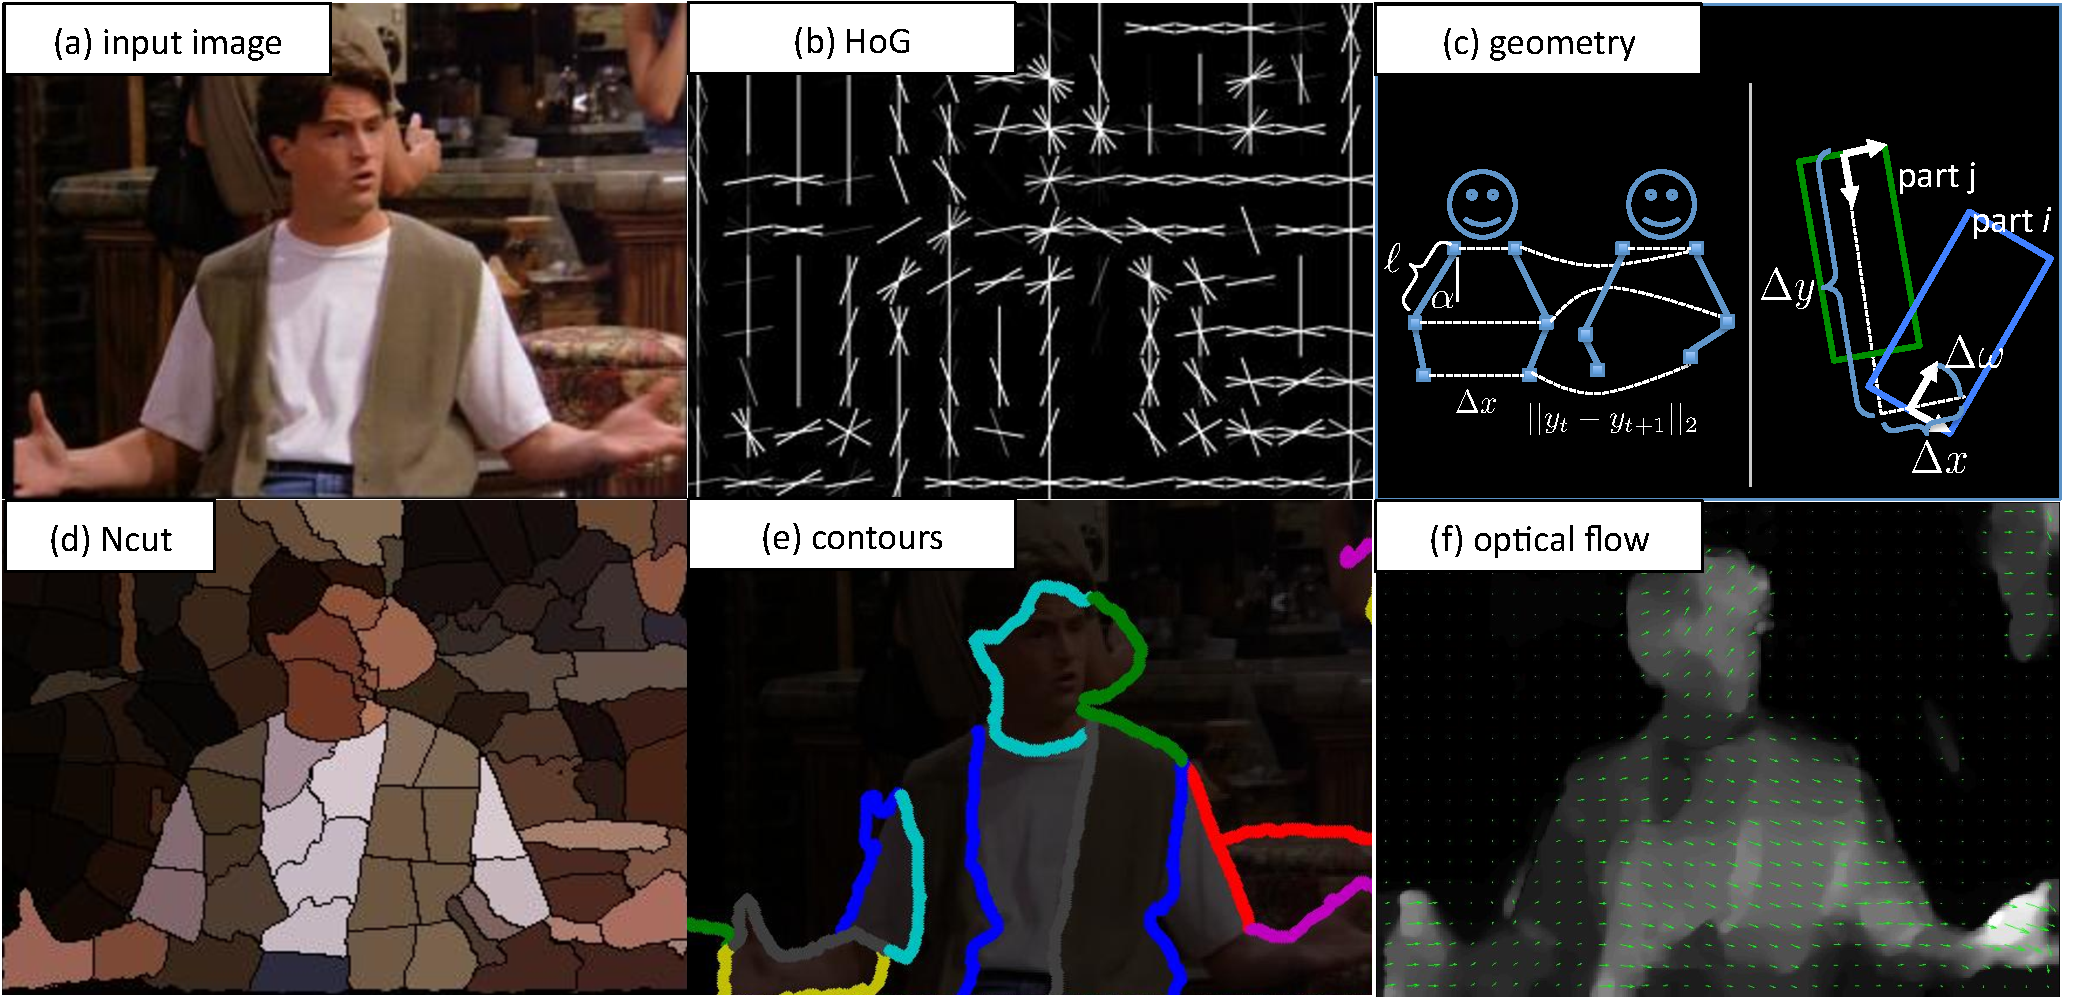
\includegraphics[width=1.05\textwidth]{figs/feature-sources.pdf}
\caption[Feature sources.]{Feature sources. (a) Running example input image.  
(b) Coarse HoG representation. (c) Different geometric quantities we compute 
for our models. (d) Normalized cuts.  (e) Long contours derived from Ncut 
segment boundaries. (f) Optical flow field shown sparsely as a quiver plot over 
the dense magnitude of the optical flow field at every pixel.}
\label{fig:feature-sources}
\end{center}
\end{figure}



\section{Edges}\label{sec:edges}
The standard cue for pictorial structures is rigid templates based on 
edges~\citep{ferrari08,eichner09,andriluka09,ddtran,devacrf,deva2011}.  Edges 
provide invariance to lighting bias and color.  Robust descriptors on top of 
edges provide additional invariance to lighting changes and slight 
translations, by coarsely binning edge magnitude and orientation, possibly with 
local edge energy normalization.  \citet{andriluka09} used Shape 
Context~\citep{belongie2001} on top of Canny edge detection for a sparse 
representation which handles angular deformation well by binning radially.  

In all our work, and many others, we use an unsigned histogram of gradients 
(HoG) descriptor, which partitions the image into a coarse uniform grid of 
cells, and measures the edge energy discretized into the uniform grid of 
spatial bins (cells) and $9$ unsigned orientation bins.  HoG was originally 
proposed by~\citet{dalal-triggs} for pedestrian detection, and has been hugely 
popular in the object recognition community as a whole, \eg~\cite{pff-dpm}.  We use a modified version of the implementation 
by~\citet{pff-dpm}, changed to use only unsigned orientations and no color.  
See~\figreff{feature-sources}{b}.

\section{Color}\label{sec:color}
Color is a tricky cue to exploit, being highly variable from image to image.  
However, having knowledge of the foreground and/or background color is powerful 
information that enables us to separate unlikely poses from likely ones---we 
can exploit such assumptions as figure/ground color separation and foreground 
constancy across the body and through time. 

\begin{figure}[tb]
\begin{center}
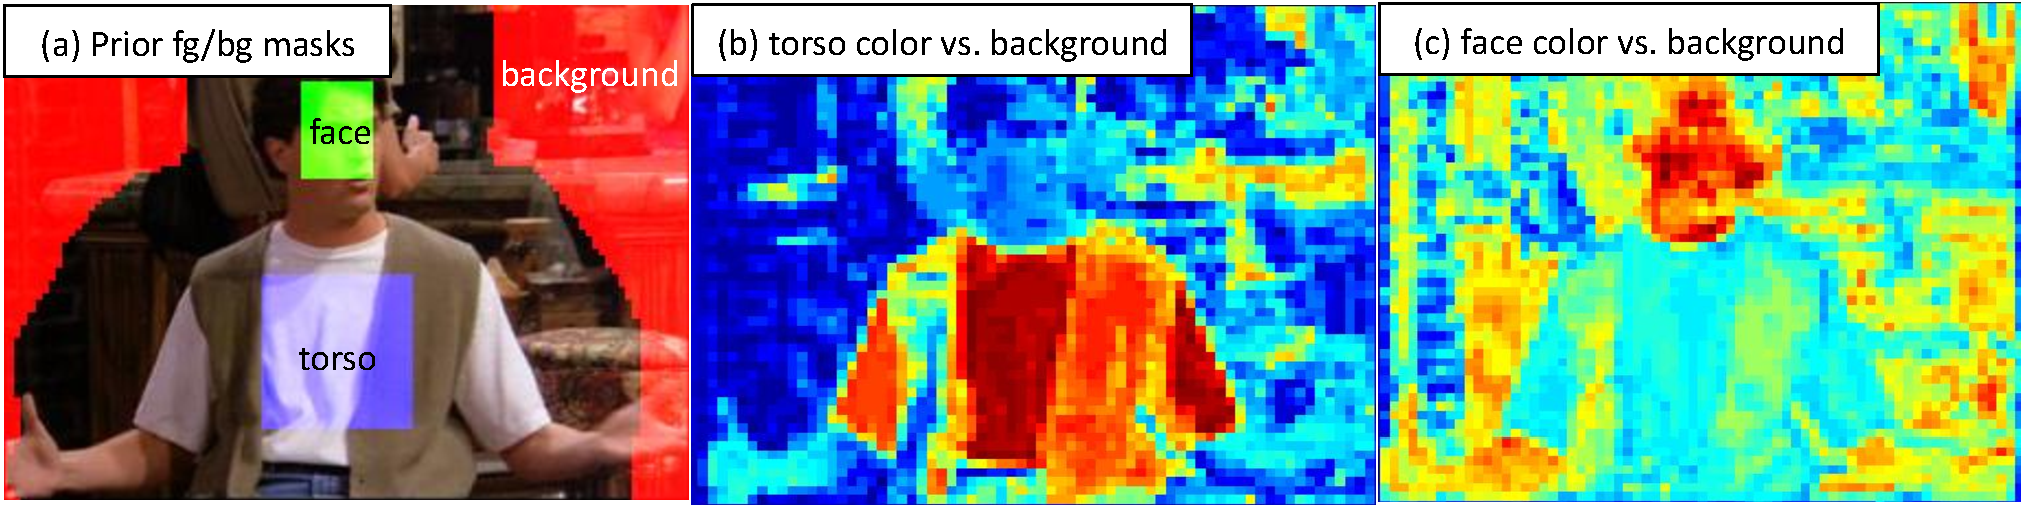
\includegraphics[width=0.99\textwidth]{figs/fg-color.pdf}
\caption[Foreground color estimation.]{Foreground color estimation.  (a) Masks 
obtained from groundtruth locations of face, torso and background {\em a 
priori}, overlaid on an example image. (b,c) Output of classifier learned to 
discriminate face versus background and torso versus background independently 
for every pixel. }
\label{fig:fg-color}
\end{center}
\end{figure}



\mypar{Foreground/Background modeling}
It is difficult to model the foreground or background color without first {\em 
knowing} where the foreground and background are---``a chicken and egg 
problem''.  Some works such as~\citet{devacrf,eichner09} focus on this issue 
directly by iteratively re-estimating color and re-estimating pose.  

We choose a simple and effective method inspired by~\citet{strikeapose} to 
obtain foreground skin and clothing color models in a single pre-processing 
step.  We exploit the fact that humans are quite well-localized by people 
detectors~\citep{ferrari08}, and assume we have samples of pixels from the 
face, torso and (importantly) background.  \figref{fg-color} shows a mask of 
pixels which we sample and corresponding labels.  Treating these samples as 
{\em groundtruth}, we model color using a supervised binary classifier 
(\secref{ml}) for skin and torso color separately, using the assumed \{face, 
torso\} pixels as positive examples, and assumed background pixels as negative 
examples.  Each pixel is its own example, classified independently.

Because we have few samples that do not completely describe the range of 
foreground and background colors, and because the feature space is relatively 
small (the space of colors), it is quite easy to overfit a discriminative 
foreground/background color model to the training samples. This leads to poor 
generalization when we apply the learned model.  Using validation data, we 
found that a scheme of learning the models using an Adaboost classifier 
composed of 10 decision trees each of maximum depth 2~\citep{esl-book} worked 
well in practice.  To complete our input foreground/background color estimation 
feature source, we apply the learned face and torso color classifiers to all 
pixels in the image independently (including the training sample pixels).

\mypar{Color similarity and tracking}
It is also useful to {\em compare } the color of parts in a relative sense, for 
the purposes of color constancy between limbs and joints within a frame and 
across time.  For this, we need a description of color and a notion of 
distances that are robust to fluctuations in lighting, hue and saturation.  
Because we are only concerned with local color similarity here (between patches 
in a single or consecutive frames), we choose a vector quantization to 
partition the colorspace into a coarse colormap.  Specifically, we choose the 
method of~\citet{heckbert1982color}---\texttt{rgb2ind($\cdot$)} in {\sc Matlab}---which 
greedily chooses bisections of RGB space to minimize variance.  This 
representation is not only robust to color fluctuations, it is also fast to 
compute and lends itself easily to robust histogram comparison distances, as 
explained below.

\section{Shape}\label{sec:shape}  Shape representations have the potential to 
model very generic yet discriminative descriptions of objects.  However, they 
have seen limited success in the object recognition community, typically 
because the representations are fragile and confounded by real-world clutter, 
\eg~\citet{shock-graphs}.  Furthermore, much of the shape community is inspired 
by the study of early biological vision and psychophysics, where the focus is 
on {\em bottom-up processing}: finding objects or pieces of objects in a 
generic way---without an explicit model of any specific object---based on 
perceptual grouping principles such as symmetry, contour continuity and
parallelism, \eg~\citet{biederman-geons}.

In contrast, the object recognition community has relied heavily on data-driven 
discriminative models on top of edge template representations~\citep{voc}, such 
as the HoG representation discussed in~\secref{edges}, and 
others~\citep{dalal-triggs,viola02,dpm}.  These models leverage powerful 
machine learning machinery to distinguish foreground from background clutter, 
but the rigid edge template representation is brittle to intrinsic deformations 
and extrinsic rotation, translation and scale.

We seek to leverage the representational power of bottom-up grouping cues in 
our top-down model of human pose.  We look at shape descriptors based on region 
and contour information.  Recently other works have focused on using purely 
bottom-up shape representations in a top-down matching framework, such 
as~\citet{toshev2010,zhu2008contour,sminch11}.  Also, some of the early work on 
human pose estimation was purely bottom-up driven, based on heuristics and 
hand-crafted rules to propose and connect limbs, \eg~\citet{mori04,praveen07}.

We choose to use Multiscale Normalized Cut (Ncut)~\citep{cour05} to obtain 
regions.  Ncut seeks a balanced partitioning of the image into meaningful 
regions via a spectral decomposition of a graph over image pixels, based on 
pairwise pixel affinities. See~\figreff{feature-sources}{d}.

We obtain long continuous contours in the image from the regions obtained by 
Ncut, as follows.  We define a graph whose nodes are all boundaries between 
Ncut segments with edges linking touching boundaries. Each contour is a path in 
this graph. To reduce the number of possible paths, we restrict ourselves to 
all shortest paths. To quantify the smoothness of a contour, we compute an 
angle between each two touching segment boundaries\footnote{The angle computed 
is between straight lines fit to the last third of each segment boundary}. The 
smoothness of a contour is quantified as the maximum angle between boundaries 
along this contour. Finally, we find among all shortest paths those whose 
length exceeds $18\%$ of the estimated person's upper body and whose smoothness 
angle is less then $45^\circ$ to obtain a final set of contours, typically 15 
to 30 per image. See~\figreff{feature-sources}{e}.

\section{Geometry}\label{sec:geom}
As discussed in~\secref{ps}, most models of human pose consider only a unimodal 
function of the displacement between parts of the form $d(y_i - y_j - 
\delta_{ij})$, where $\delta_{ij}$ is the expected displacement between parts, 
and $d(\cdot)$ is typically squared Euclidean distance in a linearly 
transformed space.  In our \CPS and Stretchable Ensembles models we are not restricted to any analytical form.  
Thus we encode features based on limb lengths (Euclidean distance in pixel 
coordinates), relative angles between parts, absolute angles that limbs make 
with the horizontal, and absolute locations of limbs and joints.  The 
``absolute'' measurements are really with respect to the detected person 
bounding box, which can be thought of as a simple virtual ``root'' part which 
is always instantiated (observed) in our models.  
See~\figreff{feature-sources}{c}.

\section{Motion}\label{sec:motion} Motion gives us cues to separate foreground 
from background, and fast moving parts (\eg, hands) from more stationary ones 
(\eg head).  When consecutive frames of video are available, we obtain motion 
estimation from optical flow.  Specifically, we use the fast implementation 
from~\citet{liu-optflow}.  See~\figreff{feature-sources}{f}.




\chapter{Features}\label{sec:features2}

There are several possible ways to organize the list of features we use in our 
systems---by model, by modality, by importance.  We choose to group them 
here by variable interactions, in keeping with the story of this thesis.  To 
make clear which features are used in which models, we mark each feature with 
[CPS] (\secref{CPS}), [ESM] (\secref{stretchable}), [LLPS] (\secref{llps}), or 
some combination of the three.

\section{Discretization}
All the features described in this chapter come in a variety of units, types 
and ranges, both categorical and real.  Typically in linear models performance 
suffers significantly when features are at very different 
scales~\citep{liblinear}.  In order to incorporate these into a linear pairwise 
MRF model in a flexible manner, we {\em uniformly discretize} all the features 
discussed, mapping them to one of $b$ bins.  When a feature is real-valued, $b 
= 10$ with bin boundaries uniformly spaced between the $10^{th}$ and $90^{th}$ 
percentile of the feature's value over the training set.  When a feature is 
categorical, $b$ is equal to the number of categories.  In all cases, each 
scalar feature gets mapped to a binary vector of length $b$, with exactly one 
entry that is $1$, indicating bin membership, and the rest $0$.   This allows 
us to learn non-linear, multi-modal mappings of scalar features, as the weights 
of each bin are unconstrained.  The sparse representation allows us to compute 
$\w_i \cdot \f_i(x,y_i)$ and $\w_{ij} \cdot \f(x,y_i,y_j)$ quickly for all 
factors.

The last stage of CPS uses its own form of discretization, by way of learning 
decision tree stumps on raw feature values in a boosting procedure.  Details 
are in \secref{impl-details}.


\section{Limb-pair features}\label{sec:limb-limb}
\mypar{Color similarity [CPS:]}: We measure the color similarity of 
kinematically-connected upper and lower arms via $\chi^2$-distance between 
histograms of quantized RGB color, described in~\secref{color}.  The histograms 
are accumulated within rectangles describing the limb extent. For histograms 
$q$ and $p$, with bins indexed by $p_i$ and $q_i$, the distance is defined as
$$\chi^2(p,q) = \frac{1}{2} \frac{\sum_i (p_i - q_i)^2}{\sum_i p_i + q_i}.$$  
We discretize the colorspace into only $8$ bins to histogram, giving us a 
stable but crude representation of color.  The coarseness of the quantization 
is permissible because we only need to model a local region of a single image 
around a detected person.


\mypar{Contour support [CPS]:} We can use the set of contours $\{c_k\}$ 
obtained as described in~\secref{shape} to define features for each pair of 
lower and upper arms, which encode the notion that those two parts should share 
a long smooth contour, which is parallel and close to the part boundaries. For 
each arm part $y_i$ and a contour $c_k$ we can estimate the edges of $c_k$ 
which lie inside one of the halves of the supporting rectangle of $y_i$ and 
whose edge normals build an angle smaller than $\omega$ with the normal of the 
part axis.  We denote the number of those edges by $q_{ik}(\omega)$.  
Intuitively, a contour supports a limb if it is mostly parallel and enclosed in 
one of the limb sides, i.e.~the value $q_{ik}(\omega)$ is large for small 
angles $\omega$. A pair of arm limbs $y_i$, $y_j$ should have a high score if 
both parts are supported by a contour $c_k$, which can be expressed as the 
following two scores
\[
  \textrm{cc}_{ijk}^{(1)}(\omega, \omega') = \frac{1}{2}\left(\frac{q_{ik}(\omega)}{h_i} + \frac{q_{jk}(\omega')}{h_j}\right)\quad\textrm{and}\quad\textrm{cc}_{ijk}^{(2)}(\omega, \omega') = \min\left\{\frac{q_{ik}(\omega)}{h_i}, \frac{q_{jk}(\omega')}{h_j}\right\}
\]
where we normalize $q_{ik}$ by the length of the limb $h_i$ to ensure that the 
score is in $[0,1]$. The first score measures the overall support of the parts, 
while the second measures the minimum support. Hence, for $y_i$, $y_j$ we can 
find the highest score among all contours, which expresses the highest degree 
of support which this pair of arms can receive from any of the image contours:
\[
\textrm{cc}_{ij}^{(t)}(\omega, \omega') = \max_{k} \textrm{ 
cc}_{ijk}^{(t)}(\omega, \omega'), \quad\textrm{for} \quad t\in\{1,2\}
\]
By varying the angles $\omega$ and $\omega'$ in a set of admissible angles 
$\Omega$ defining parallelism between the part and the contour, we obtain 
$|\Omega|^2$ contour features\footnote{We set $\Omega=\{10^\circ, 20^\circ, 
30^\circ\}$, which results in $18$ features for both scores.}  The features are 
illustrated in~\figreff{contour-feature}{(b)}.

\mypar{Geometry [CPS]:} We measure the interior angle made between parts, 
keeping the part identity so that the angle is in the full range $[0,2\pi]$.  
We also look at difference from the expected position $\delta_{ij}$ for a pair 
of parts, using the signed $x$ and $y$ components as features.

\begin{figure}[tb]
\begin{center}
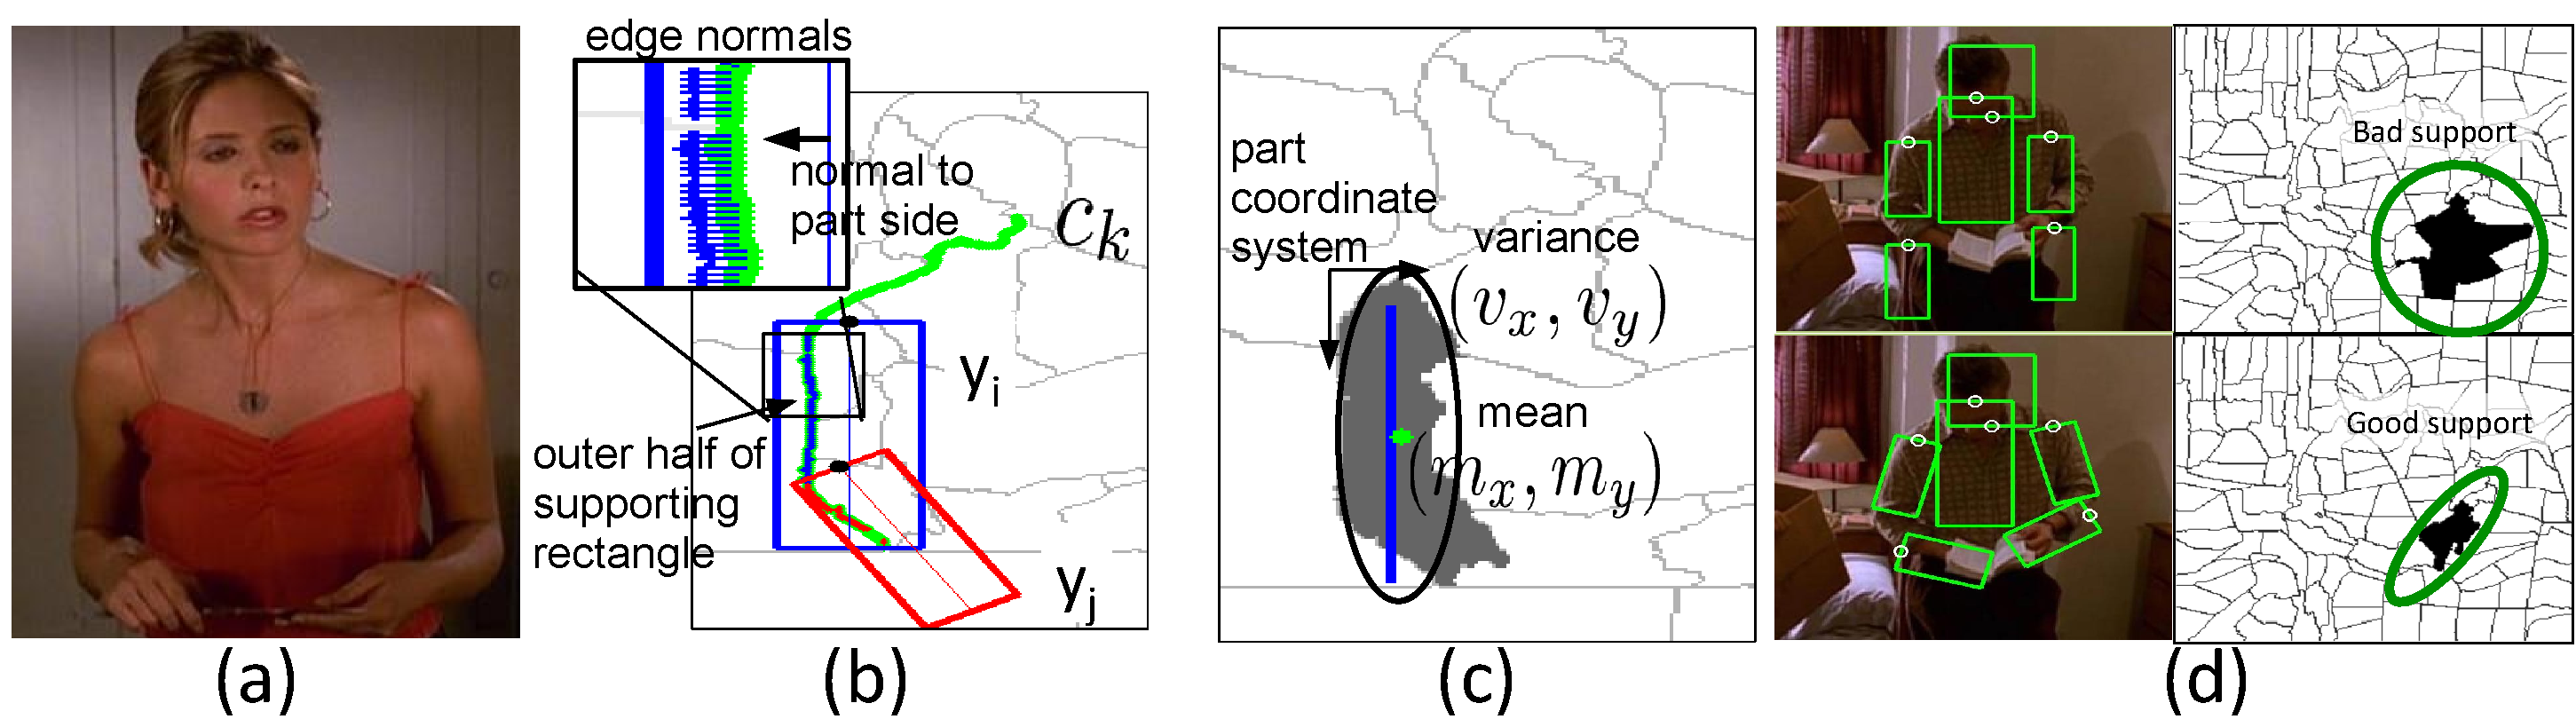
\includegraphics[width=0.99\textwidth]{figs/contour-feature.pdf}
\caption[Shape features.]{Shape features.  (a) Input image.  (b) Measuring a 
pair of limbs co-likelihood by checking attachment to long contours in the 
image, as described in the ``Contour support'' feature.  (c)  Measuring the 
likelihood of a single limb's region support, as described in the ``Region 
support'' feature. (d) Examples of right lower arm hypotheses that have poor 
support from underlying regions (top), and good support (bottom).}
\label{fig:contour-feature}
\end{center}
\end{figure}


\section{Joint-pair features}\label{sec:joint-joint}
\mypar{HoG limb detectors [CPS, ESM]:} For each of the 6 body parts -- head, 
torso, upper and lower arms -- we learn an individual Gentleboost 
classifier~\cite{friedman00} on HoG features (\secref{edges}) using the Limbs 
Annotated in Movies Dataset\footnote{LAMDa is available at 
\textit{http://vision.grasp.upenn.edu/video}}.  We then apply these detectors 
densely over all orientations and locations and downsample by max-pooling or 
upsample via nearest-neighbor to get a heatmap of beliefs over our state space.

\mypar{Region support [CPS, ESM]:}
We compute the first and second order moments of the segments lying under the 
major part axis\footnote{We select segments which cover at least $25\%$ of the 
part axis.} to coarsely express shape of limb hypotheses as a collection of 
segments $R$, the union of all segments that support the part hypothesis. To 
achieve rotation and translation invariance, we compute the moments in the part 
coordinate system.  We include convexity information $|conv(R)|/|R|$, where 
$conv(\cdot)$ is the convex hull of a set of points, and $|R|$ is the number of 
points in the collection of segments.  We also include the number of points on 
the convex hull, and the number of part axis points that pass through $R$ to 
express continuity along the part axis.  See~\figreff{contour-feature}{b,c}.

\mypar{Foreground color [CPS, ESM]:} Using likelihood heatmaps of estimated 
skin and torso color (\secref{color}), we measure the likelihood that a limb is 
present at a particular location by a mean heatmap value inside the rectangular 
extent of a part, for each color model (face and torso). This can be computed 
efficiently densely via convolution with an all-ones filter, separable over 
dimensions, for each orientation.  If desired, the feature can be computed 
efficiently over a sparse set of locations using integral 
images~\citep{viola02}.

\mypar{Geometry [CPS, ESM, LLPS]:} To describe the geometry of a limb in CPS, 
we use as features its absolute position and orientation with respect to the 
image axes.  Position is discretized into a coarse spatial grid, and 
orientation is discretized into 24 possible values; both categorical features.

In the Stretchable Ensemble Model, we use the following pairwise geometric 
features for limbs in a single frame: (i) length of arms, (ii) unsigned 
difference in angle that the upper arm makes with respect to the vertical axis, 
(iii) difference in x-coordinate between left-right symmetric joints, from 
which our model can learn a type of repulsion behavior (e.g., the left shoulder 
should be far from the right shoulder) as well as a left-right order of parts 
(e.g., the left shoulder should be to the left of the right shoulder). Note 
that we do {\em not} express features describing the angle of the lower arm, 
leaving it free to rotate and stretch.
See~\figreff{misc-features}{d}.

To express joint motion continuity through time in ESM, we use one simple 
geometric feature: the Euclidean distance between the joint in consecutive 
frames, discretized into 10 binary values.   In LLPS, we use standard quadratic deformation features as in~\secref{dt} \citep{felz05}.

\mypar{Contour support [ESM]:}  For each arm joint-pair, we measure its support 
from long contours extracted in the image (~\secref{shape}) as follows: we take 
the number of contour points that are roughly parallel to the joint-pair line 
segment (angle less than $12^\circ$) and within a spatial support region 
(approximately 25\% of the length of the average limb).  We then use as a 
feature the number of supporting contour points, normalized by the length of 
the limb hypothesis.  Due to the sparse contour set, this feature can be 
computed extremely efficiently, by quickly discarding hypotheses whose 
endpoints are not near any contour.  See~\figreff{misc-features}{c}.

\mypar{Color consistency [ESM]:} To capture the fact that the color of pairs of 
joints is often similar due to clothing and/or skin color, we describe the 
color consistency of pairs of joints via the $\chi^2$-distance between color 
histograms obtained from small image patches (with side length 10\% of image 
dimensions) extracted around each joint.  See~\figreff{misc-features}{b}.

\mypar{Color tracking [ESM]:}  We capture the persistence of appearance over 
time with a simple and effective patch-based color tracker for each joint.  We 
jointly quantize each pair of consecutive images into a small number of color 
indices, using minimum variance quantization (\secref{color})---here with 32 
colors.  We then compare patches (of side length 10\% of the image dimensions) 
around the joint in each frame using an $L_0$-norm (Hamming loss) distance 
function:  Let $P_{t}$ and $P_{t+1}$ represent quantized color image patches 
around the joint in frame $t$ and $t+1$, with $N$ pixels.  Then the color 
tracking distance feature is $ 
||P_t~-~P_{t+1}||_0~=~\frac{1}{N}~\sum_{(r,c)}~\Ind[P_{t}(r,c)=P_{t+1}(r,c)]$ 
where (r,c) indexes rows and columns in the patch.  
See~\figreff{misc-features}{b}.

The coarse quantization gives us a robust way to compare the color in 
consecutive frames that is tolerant to changes in lighting and pixel 
fluctuation.  The $L_0$ distance is more robust than Euclidean distance/radial 
basis similarity scores often used (\eg~\citet{gould08ijcv}), in which the 
distance grows with the distance in the color space and can thus be corrupted 
by a few large outlying pixels.  Furthermore, it is a much more discriminative 
cue than color histogram distances across time (as used in \eg~\citet{ren07}) 
because it requires that the {\em pixel structure} of the patch be similar in 
consecutive frames.  

\mypar{Figure from flow [ESM]:}
We use several features based on dense optical flow from~\cite{optflow}, which we compute between 
adjacent frames. We obtain a rough estimate of the foreground of each clip by 
assuming there are only 2 planes of motion: foreground (figure) and background.  
Given a detected person, we estimate the background motion by computing the 
median flow vector $\mu_{bg}$ outside the detected person bounding box, and not 
considering outlier flow with magnitude greater than the $75^{th}$ percentile.  
We then subtract off $\mu_{bg}$ from the flow field and take the magnitude of 
the flow as an estimate of foreground likelihood.  We incorporate this as a
limb feature by computing the average foreground likelihood sampled at 5 points 
evenly spaced along the line segment between joint pairs.
See~\figreff{misc-features}{e}.

\section{Single joint features} \label{sec:single-joint}

\begin{figure}[tb]
\begin{center}
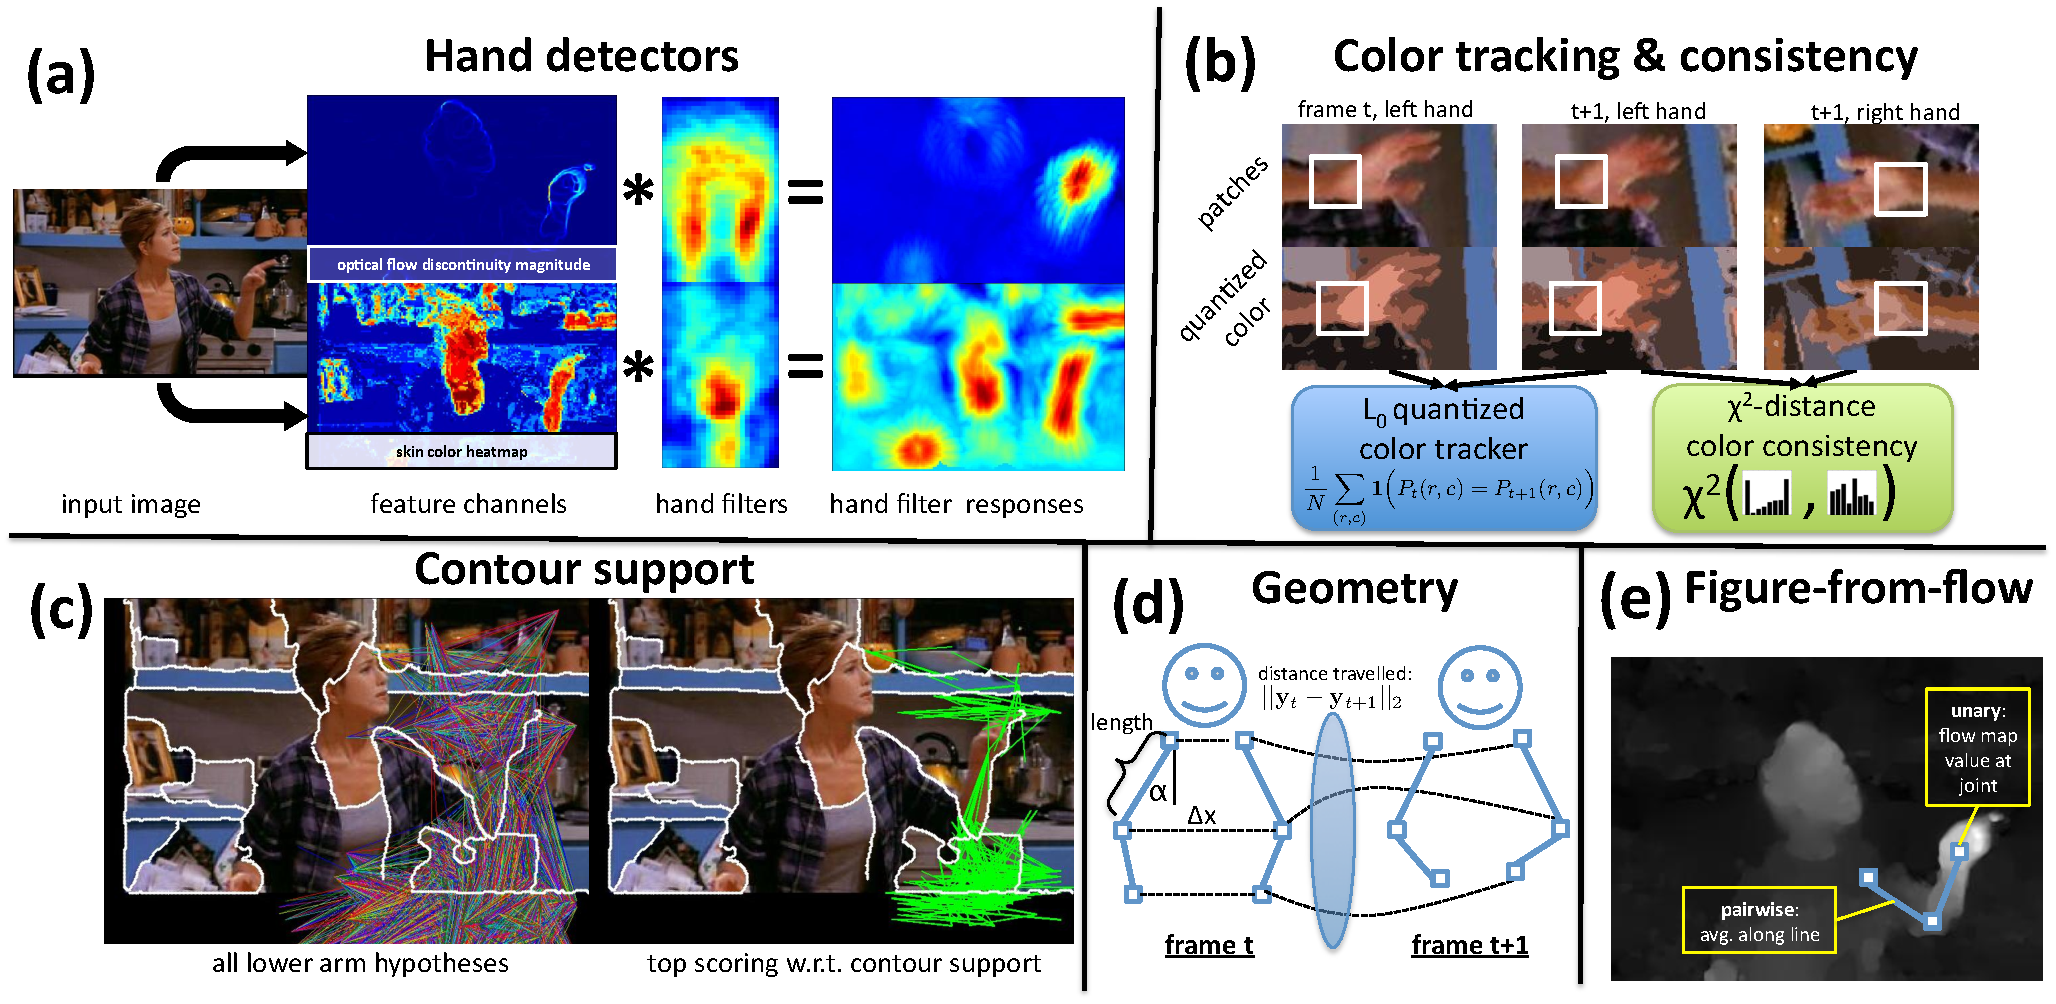
\includegraphics[width=0.99\textwidth]{figs/misc-features.pdf}
\caption[Joint and joint-pair features.]{Joint and joint-pair features. See 
\secref{joint-joint} and \secref{single-joint}. (a)  Hand detectors.  (b) Color 
distances for left-right symmetry and tracking, using a quantized color space 
(shown).  (c) Visualization of arm hypotheses that are supported by contours in 
the image.  (d) Joint-joint geometry we employ in our Stretchable Ensemble 
model.  (e)  Figure-ground estimation by estimating two flow clusters.}
\label{fig:misc-features}
\end{center}
\end{figure}


\mypar{Histogram of Gradients [ESM, LLPS]:} 

In ESM we have no specific learned model of joints, so we project down trained 
limb detectors from~\secref{joint-joint}, taking a max over all possible angles 
and over 3 possible limb lengths (not foreshortened, somewhat foreshortened, 
extremely foreshortened; estimated by quantiles of dataset groundtruth limbs).

In LPPS, we represent joints with $5 \times 5$ cell Histogram of Gradients 
descriptors around each joint, using the implementation from~\cite{dpm}, 
modified to use only 9 un-signed edge orientations.  Using these features, 
learned parameters capture the local shape around each joint, {\em specific to} 
the variations of pose and appearance in a small local neighborhood.  We 
supplement the HoG channels with an extra ``out-of-image'' channel, to jointly 
learn if it's likely that a body part lies at least partially outside the image 
coordinates.

\mypar{Color and motion-based hand detectors [ESM]:}  Detecting the hand 
location is an extremely useful cue in anchoring all joint locations.  
Unfortunately, traditional template-based part detectors such as HoG detectors 
fail at this task due to hands' high variability in appearance, pose, and 
motion blur.  We instead learn discriminative linear filters~\citep{liblinear} 
from two different input modalities:  (1) Skin detection heatmaps.  
(\secref{color}).  (2) The gradient of the magnitude of the optical flow field 
between consecutive images (\secref{motion}).  The latter exploits the fact 
that hands are often in motion (and naturally the fastest moving body part).  
Both linear filters can be evaluated efficiently densely via convolution.  
See~\figreff{misc-features}{a}.

\mypar{Figure from flow [ESM]:}
We again use an estimate of foreground via optical flow magnitude as 
in~\secref{joint-joint}, and \figreff{misc-features}{e}.  Here we report a mean 
foreground likelihood in a small window around the joint as a feature.
